%===============================================================================
%      Introduction
%===============================================================================
\section{Introduction}

   Nous allons ici voir comment en arriver à un noyau présent dans la
mémoire de la machine, prêt à être exécuté. La procédure peut varier
d'un système à l'autre : le code peut être sur un support amovible,
dans une zone mémoire non volatile, sur une machine distante, \ldots


   Dans les cas les plus simples, l'auteur du noyau n'a (presque) pas
à s'en préoccuper, dans les cas les plus tordus, il ou elle va devoir
(presque) tout faire. Nous décrirons ici deux variantes :

\begin{itemize}
   \item Nous commencerons par nous fonder sur une situation ``à
     l'ancienne'' avec un PC doté d'un lecteur de
     disquettes. Nous utiliserons alors le \bios du \pc
     pour charger le noyau en mémoire, lui passer quelques
     informations et le faire démarrer.

     Dans cette situation, nous devrons donc (presque) tout faire
     puisqu'il va falloir aller charger le noyau depuis la disquette
     vers la mémoire. Heureusement le \bios nous fourni des fonctions
     pour cela.

   \item Nous observerons ensuite des outils un peu plus modernes
     permettant de démarrer de façon un peu plus simple et plus
     indépendante du matériel sous-jacent.

     Dans cette situation, nous utiliserons par exemple {\tt grub} qui fera
     le travail de charger le noyau depuis le support (disque dur,
     \ldots) vers la mémoire. Nous aurons juste quelques informations
     à lui fournir.
  
\end{itemize}

%===============================================================================
%
%===============================================================================
\section{Démarage à partir d'une disquette}

   Nous allons donc devoir mettre en \oe{}uvre le boot du noyau dans
cette configuration. Pour cela, nous allons construire un fichier qui
sera placé sur une disquette à partir de laquelle notre système pourra
démarrer. Notons que nous utiliserons ici un émulateur comme Qemu ou bochs
auquel nous donnerons le chemin vers ce fichier et à qui nous
demanderons de démarrer depuis cette disquette. Mais nous pouvons
également copier ce fichier sur une disquette pour démarrer une vraie
machine.

   La première étape d'un tel démarrage est assuré par le système
lui-même : il s'agit de récupérer notre code sur la disquette, le
mettre en mémoire puis lui donner la main. C'est le BIOS qui va faire
cela. Malheureusement, son action est assez limitée, et il ne va
charger que 512 octets en mémoire. De ce fait,
notre code doit, d'une part être d'une taille inférieure à 512 octets
et d'autre part charger en mémoire le noyau lui-même.

   Nous allons donc construire un fichier composé essentiellement de
trois parties :

\begin{itemize}
     \item un {\em secteur de boot} (ou {\em bootsector}) sera un code
       de moins de 512 octets qui va s'occuper de charger le noyau ;
     \item un code d'initiaisation qui va préparer le terrain pour le
       noyau avant de démarrer celui-ci ;
     \item le noyau lui-même.
\end{itemize}

   Observons la structure de ce fichier pour ManuX puis regardons comment en
construire chaque partie.

%-------------------------------------------------------------------------------
%
%-------------------------------------------------------------------------------
\subsection{Construction du fichier de démarrage}

   Afin de permettre un démarrage ``à l'ancienne'' par un boot sur
disquette du \textsc{ pc}, nous allons donc construire une image de disquette
dont la structure est décrite par la figure suivante.

   Le code d'initialiation est ici nommé {\tt initmanux}. Je fais figurer
à la fin du noyau un fichier appelé {\tt ramdisk} qui peut être
présent et comporté un premier système de fichiers élémentaire.

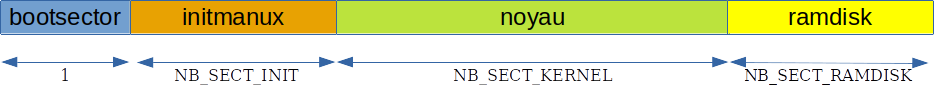
\includegraphics{images/image-disquette.png}

%\begin{figure}
%  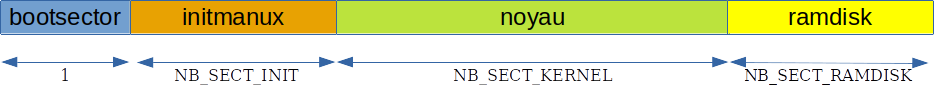
\includegraphics{images/image-disquette.png}
%\caption{\label{fig:image-disquette}Le fichier de démarage}
%\end{figure} 

   Ce que j'appelle ici le boot du système se passera donc en deux
temps. D'abord le secteur de boot est chargé en mémoire par le
\bios qui lui donne la main.

   Le secteur de boot  s'occupe alors de charger en mémoire le code
d'initialisation ainsi que le code du noyau. Il donne alors à son tour
la main à l'initialisation. Ce second élément réalise quelques
opérations puis démarre enfin le noyau.

   Si le secteur de boot et le code d'initialisation sont deux
éléments distincts, c'est pour deux raisons principales

\begin{itemize}
   \item d'une part le secteur de boot ne dispose que de 512 octets,
     si bien qu'il doit être réduit au  minimum ;
   \item chacun de ces deux éléments à un rôle bien spécifique
     (charger le code en mémoire et initialiser le système).
\end{itemize}

   Avant de regarder en détail comment ils sont mis en \oe{}uvre,
regardons les interactions entre les trois éléments.
   
%-------------------------------------------------------------------------------
%
%-------------------------------------------------------------------------------
\subsection{Liens entre les trois éléments}

   Les trois parties de codes évoquées ici (le secteur de boot, le
code d'initialisation et le noyau) ne sont pas liées entre elles (par
une édition de liens). Les appels de fonction, partages de variables,
\ldots {} sont alors à éviter car peu pratiques !

   Concrètement, il y a surtout deux ``appels de fonction'' à réaliser : 

\begin{itemize}
   \item le secteur de boot doit lancer le code d'initialisation ;
   \item le code d'initialisation doit démarrer le noyau.
\end{itemize}

   Pour cela, on va utiliser le fait que tous les éléments sont
placés à des adresses connues et faire un saut à ces adresses.
   
%-------------------------------------------------------------------------------
%
%-------------------------------------------------------------------------------
\subsection{Le secteur de boot}

   Lorsqu'on allume un \textsc{ pc} normalement configuré avec une disquette dans
le premier lecteur, le \textsc{ bios} charge le premier secteur de la diquette en
mémoire et l'exécute. En fait, il ne fait cela que si les deux derniers octets
de ce secteur contien\-nent la valeur magique {\tt 0xAA55}. Pour être
plus précis, c'est à l'adresse {\tt 0x7C00} que ce secteur est chargé.

   Un secteur étant composé traditionnellement de 512 octets, on ne
peut pas faire des folies avec le secteur de boot ! On va donc se
contenter de charger en mémoire d'autres secteurs du disque. Pour
cela, on peut utiliser le \bios et plus particulièrement
l'interruption 13h qu'il nous fournit pour manipuler les lecteurs.

   Le secteur de boot de ManuX est codé dans le fichier
\lstinline!boot/bootsector.nasm! et il est donc écrit en \nasm. Il est
très simple et se contente d'utiliser le \bios pour charger le
noyau en mémoire puis de faire un saut au début de la mémoire ainsi
initialisée.

   Il n'est pas très robuste, en particulier sur la taille attendue du
noyau et sur l'adresse à laquelle le placer !

   Concrètement, ce chargement se fait en deux phases :

\begin{itemize}
   \item Chargement du code d'initialisation : c'est le code qui va
     avoir pour rôle d'initialiser le système. Ce code est écrit en
     assembleur dans le fichier \lstinline!boot/init-manux.nasm!.
   \item Chargement du code du noyau : c'est tout le code de ManuX qui
     est ici chargé en mémoire. Il sera exécuté par le code
     d'initialisation. 
\end{itemize}

   Après ces deux chargements, le code du secteur de boot exécute le
code d'initialisation.

   Je ne décris pas plus ce code qui ne présente pas un intérêt
profond, les plus curieuses et curieux n'ont qu'à lire le code ! Vous
pourrez le trouver dans le fichier \fichier{boot}{bootsector}{nasm}.
   
%-------------------------------------------------------------------------------
%
%-------------------------------------------------------------------------------
\subsection{État de la mémoire après le chargement}

   L'état de la mémoire à la fin du boot est décrite par la figure
suivante. Les nombres sous les différentes zones expriment leur taille
en nobre de pages (la taille d'une page est de 4 Ko). Les macros sont
définies dans le fichier de configuration de \manux :
\fichier{include/manux}{config}{h}.

\includegraphics{images/etat-memoire-boot.png}

%\begin{figure}[htbp]
%\includegraphics[width=\textwidth]{etat-memoire-boot}
%\caption{\label{fig:etat-memoire-boot}État de la mémoire après le boot}
%\end{figure} 

   Une fois qu'il a terminé son travail, le code du secteur de boot
donne la main au code d'initialisation.
   
%-------------------------------------------------------------------------------
%      L'initialisation
%-------------------------------------------------------------------------------
\subsection{L'initialisation}

   Le "programme" d'initialisation est traditionnellement consacré à la détection
et à l'initialisation (original, vu son nom !) du matériel. Sur un \pc de
base, on peut là encore se faire aider du \bios. 

   En ce qui concerne \manux, cette phase d'initialisation va profiter
du fait qu'elle n'a pas les mêmes limites de taille que le secteur de
boot (un seul secteur comme le nom au singulier le suggère). On va
donc pouvoir y réaliser certaines actions un peu plus confortablement,
comme :

\begin{itemize}
   \item vérifier la mémoire disponible (cette information sera passée au
     noyau) ; 
   \item passer en mode protégé ;
   \item charger en mémoire un ramdisk qui nous permettra de jouer avec
    des systèmes de fichiers  sans avoir besoin d'implanter la gestion
    de matériel.
\end{itemize}

   Voyons rapidement quelques points.

%...............................................................................
%      Passage en mode protégé
%...............................................................................
\subsubsection{Passage en mode protégé}

   Les processeurs Intel démarre dans un mode de fonctionnement appelé
le {\em mode réel} (real mode). Dans ce mode, la mémoire est accédé de
façon linéaire. En mode protégé, l'utilisation de la mémoire est un
peu plus complexe (mais également plus puissante). Je ne vais pas
rentrer dans les détails ici, vous trouverez énormément de
documentation sur le sujet, par exemple les manuels Intel !

   Le basculement du mode réel vers le mode protégé n'est pas
immédiat, il nécessite un peu de travail.
   
%...............................................................................
%      Passage des informations au noyau
%...............................................................................
\subsubsection{Passage des informations au noyau}

   La plupart des informations recueillies par l'initialisation peuvent se
révéler particulièrement intéressantes pour le noyau. Il est donc important de
se définir un mécanisme permettant de faire passer ces informations depuis la
phase d'initialisation jusqu'au noyau.

   Nous allons utilise deux registres pour faire passer de
l'information au noyau :

\begin{itemize}
   \item Le registre \lstinline!eax! contiendra un ``nombre magique'',
     c'est-à-dire une valeur prédéfinie permettant au noyau
     d'identifier avec une bonne confiance le {\em bootloader}
     utilisé.
   \item Le registre \lstinline!ebx! contiendra l'adresse d'une
     structure dans laquelle seront enregistrées les différentes
     informations vraiment utiles pour le noyau.
\end{itemize}

   (Notons que ce choix (tout comme la structure qui va suivre) est
largement inspiré du fonctionnement de {\em Multiboot}). Nous aurons
donc par exemple la définition suivante dans le fichier
\fichier{include/manux}{multiboot}{h} 

\lstset{language=C}
\begin{lstlisting}
typedef struct _InfoSysteme {
   uint32_t flags;           // Pour compatibilité avec multiboot
   uint32_t memoireDeBase;   // En Ko
   uint32_t memoireEtendue;  // En Ko
   uint32_t peripheriqueDemarrage ;
   char *   ligneCommande;
} InfoSysteme;
\end{lstlisting}

   Naturellement, pour que tout cela fonctionne, il est nécessaire, à la fin
de la phase d'initialisation, d'initialiser correctement ces
registres. Voici donc par exemple à quoi peuvent ressembler les
dernières lignes de la phase d'initialisation :

\lstset{language=nasm}

\begin{lstlisting}
        ; On passe au noyau quelques infos
        ;---------------------------------
        mov eax, MANUX_INIT_MAGIC
        mov ebx, InfoSysteme

        ; Et c'est parti, on saute sur le noyau !
        ;----------------------------------------
        jmp MANUX_KERNEL_START_ADDRESS  
\end{lstlisting}

   Notons que, bien sûr, aucun contôle de type ne peut être fait entre les deux
phases et qu'il est donc important que le programmeur définisse de façon
cohérente la structure C et la zone mémoire gérée en assembleur.

%...............................................................................
%      Détection de la mémoire
%...............................................................................
\subsubsection{Détection de la mémoire}

   En ce qui concerne cette détection, nous allons encore une fois
utiliser un service du \bios, au travers de l'interruption 0x12 qui va
nous fournir ces informations.

   Vous trouverez le code correspondant dans le fichier
\fichier{boot}{init-manux}{nasm}. 


%===============================================================================
%
%===============================================================================
\section{Utilisation de {\em Multiboot}}

   Nous allons ici utiliser la spécification {\em Multiboot} définie
par la {\em Free Software Foundation} qui va nous permettre d'utiliser
les services d'outils tels que GRUB afin de grandement simplifier
le chargement du noyau de ManuX.

   Cela nous permettra également d'utiliser des outils un peu plus
modernes qu'un lecteur de disquettes et, par voie de conséquence, de
faire fonctionner ManuX sur autre chose que des machines virtuelles ou
hors d'age !

%-------------------------------------------------------------------------------
%
%-------------------------------------------------------------------------------
\subsection{Structure du fichier chargé par {\em Multiboot}}

   Nous devons construire un fichier qui sera fourni à {\em
Multiboot}.  Nous allons utiliser ici la version 1 de {\em Multiboot} et
non {\em Multiboot2}. On trouvera la spécification par exemple
\href{ici}{https://www.gnu.org/software/grub/manual/multiboot/multiboot.html}.

   Un tel fichier contient essentiellement notre noyau, mais doit avoir
une structure particulière afin d'être pris en charge~:

\begin{itemize}
   \item Il doit être composé d'un entête suivi d'un programme
     exécutable.
   \item L'entête, qui permet à l'outil de boot (comme {\sc grub})
     d'identifier le fichier, a une structure bien définie, que nous
     allons décrire ci dessous. Il doit être dans les 8192 premiers
     octets du fichier.
   \item Le programme exécutable peut être à n'importe quel format. Il
     doit évidemment être ``auto-suffisant'' (pas de librairies
     dynamiques !). Il doit pouvoir être positionné à n'importe quelle
     adresse physique en mémoire. 
\end{itemize}

   Le programme exécutable, c'est évidemment ManuX. Nous allons
décrire maintenant la structure de l'entête.
     
%-------------------------------------------------------------------------------
%
%-------------------------------------------------------------------------------
\subsection{Structure de l'entête}

   Le système {\em Multiboot} nécessite donc un entête devant le noyau
avec des caractéristiques bien définies.


%-------------------------------------------------------------------------------
%
%-------------------------------------------------------------------------------
\subsection{L'entête de ManuX}

   En ce qui concerne ManuX, il est
implanté dans le fichier \fichier{boot}{mb-manux}{nasm}.

   Ce fichier contient essentiellement quelques éléments permettant à
{\em Multiboot} de le reconnaitre puis du code permettant de démarrer
véritablement le noyau par un appel à la fonction \lstinline!_start()!
qui sera implantée dans le fichier \fichier{noyau}{main}{c}.

%-------------------------------------------------------------------------------
%
%-------------------------------------------------------------------------------
\subsection{Réalisation d'une image {\sc iso}}

   La cible {\tt iso}  du {\tt Makefile} principal permet de générer
un fichier {\sc iso} qui peut être utilisé pour démarrer ManuX sur une
machine physique ou virtuelle.

   La cible {\tt multiso} du {\tt Makefile} principal permet de
générer une image {\sc iso} intégrant un noyau pour chaque fichier de
configuration présent dans le répertoire {\tt multiconf}.

%===============================================================================
%
%===============================================================================
\section{Démarrage du noyau}

%-------------------------------------------------------------------------------
%
%-------------------------------------------------------------------------------
\subsection{Démarrage du noyau ({\tt noyau/main.c})}

   La dernière action du programme d'initalisation est donc l'exécution
de la fonction \lstinline!_start()!. Comme je l'ai dit précédemment,
il ne s'agit pas d'un appel de foncion C classique, puisque les deux
morceaux de code ne sont pas liés entre eux, mais d'un saut à
l'adresse de la fonction (le tout après avoir empilé les paramètres).

   Ceci termine donc la description de toute la quincailleire qui nous
permet d'arriver au début de l'exécution du code du noyau. Nous allons
commencer la description de ce dernier par la mise en place des outils
de base dont il aura besoin.

%-------------------------------------------------------------------------------
%
%-------------------------------------------------------------------------------
\subsection{Obtention des paramètres passés par le {\em bootloader}}

